\documentclass{beamer}

\usepackage[utf8]{inputenc}
\usepackage{graphicx}

\title{Case Study 1-Group 1}
\author{Melody Jiang, Irene Ji, Keru Wu}
\institute{Department of Statistical Science, Duke University}
\date{01/21/2019}

\begin{document}

\frame{\titlepage}



%%%%%%%%%% Section1: Introduction %%%%%%%%%%%


\begin{frame}
\frametitle{Introduction}

\begin{itemize}
\item Data: A study by Longnecker et al. (2001), comprised of 2380 observations of pregnant women.
  
\item Goal: Assess how DDE and PCBs relate to risk of premature delivery.

\end{itemize}

\end{frame}






%%%%%%%%%% Section2: Materials & Methods %%%%%%%%%%%

\begin{frame}
\frametitle{EDA and Preprocessing}
\begin{itemize}
\item Premature delivery: Gestational Age $\leq$ 36.
\item Standardize continuous variables.
\item Missing data: Multivariate Imputations by Chained Equations (MICE package in R) for covariates. Deleted albumin because 93 percent missing. Only one observation missing in dde and pcb, deleted.
\item Limit of Detection (LOD): Exists in some PCBs. All LODs are negligible compared to data scale (e.g. 0.01 compared to 0.3)
\end{itemize}
\end{frame}




\begin{frame}
    \frametitle{EDA and Preprocessing: Collinearity and Dimensionality Reduction}

    \begin{itemize}
        \item There are 11 types of PCBs, some of which have high correlation and might distort modeling result.
          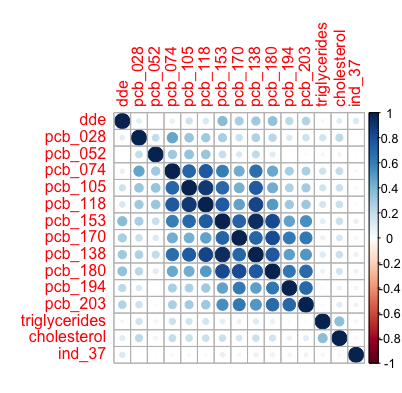
\includegraphics[scale=0.4]{corrplot.png}
        \item Possible approaches: Simple sum, PCA, Factor Analysis.
    \end{itemize}

\end{frame}

\begin{frame}
    \frametitle{EDA and Preprocessing: Collinearity and Dimensionality Reduction}

    \begin{itemize}
        \item Possible approaches: Simple sum, PCA, Factor Analysis.
         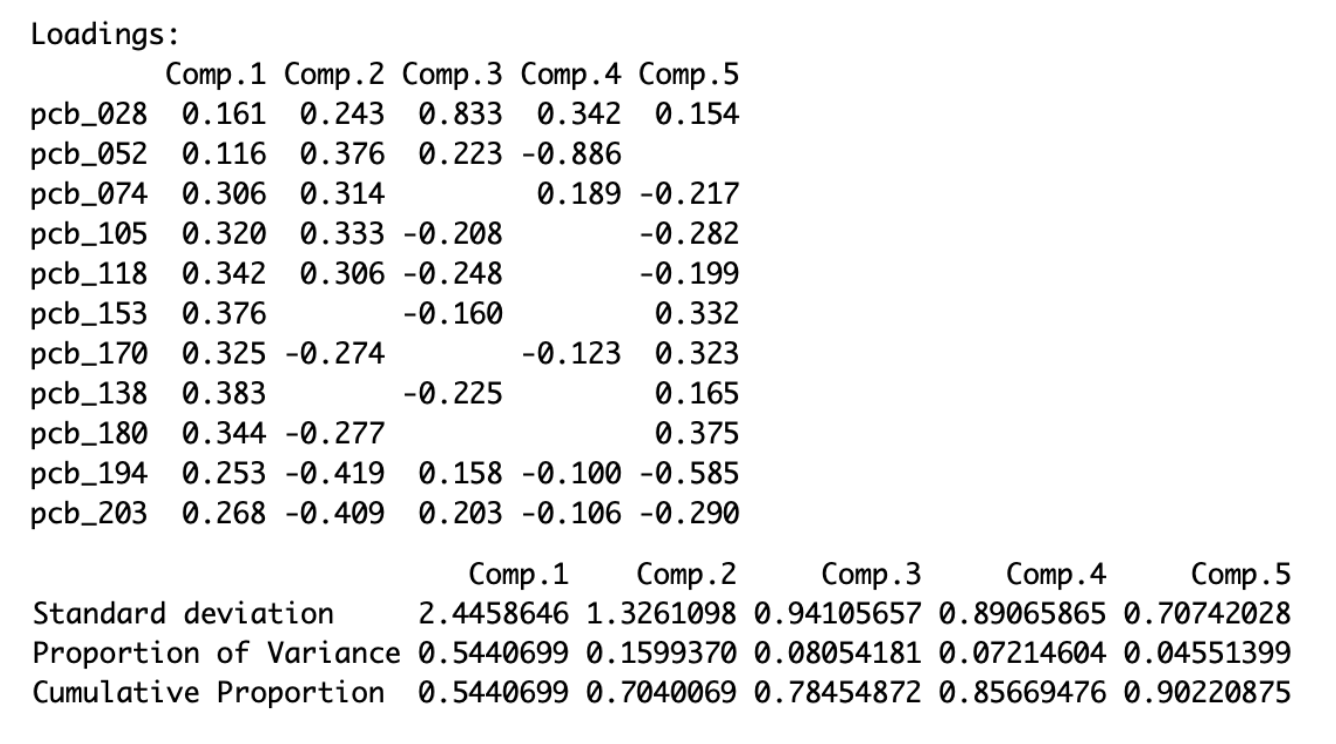
\includegraphics[scale=0.4]{PCA.png}


    \end{itemize}
\end{frame}


\begin{frame}
    \frametitle{EDA and Preprocessing}

    
    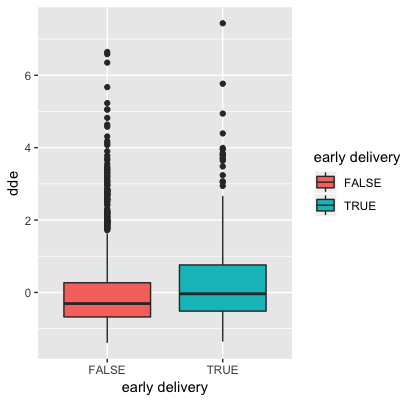
\includegraphics[width=0.49\textwidth]{ddeVSearly.png}
    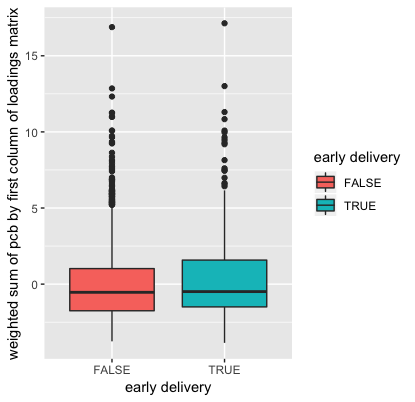
\includegraphics[width=0.49\textwidth]{pcbVSearly.png}
    
        
\end{frame}




\begin{frame}
\frametitle{Model}


\begin{itemize}
\item Binary response: use logistic regression?
\pause
\item Domain knowledge about chemical effects?
\pause
\item No effect when concentration is below some lower bound.
\pause
\item Constant effect after reaching some upper bound.
\pause
\item Generalized Additive Model (GAM)
\end{itemize}
\end{frame}


\begin{frame}
\frametitle{Model}

\begin{itemize}
\item Generalized Additive Model (GAM)
$$g(Y_i) = \beta_0 + \sum_{j=1}^m f_i(x_{ij}) + \sum_{k=1}^l \beta_{k}z_{ik}$$

\item Choice of $g$: probit or logit.
\item $x_{.j}$s include numeric variables: DDE, Principal Components of PCBs (PC1-4), Maternal Age, etc.
\item $z_{.k}$s include categorical variables.

\end{itemize}
\end{frame}



\begin{frame}
\frametitle{GAM Outputs}
\centering
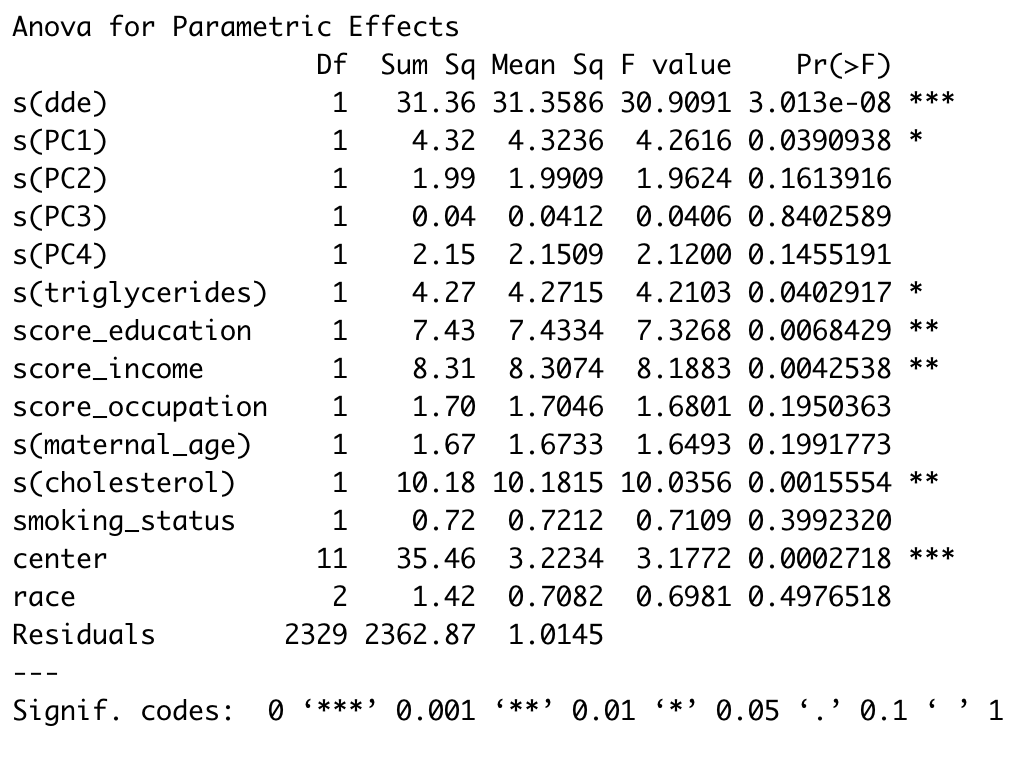
\includegraphics[width=10cm]{GAMOutputs1.png}
\end{frame}

\begin{frame}
\frametitle{GAM Outputs}
\centering
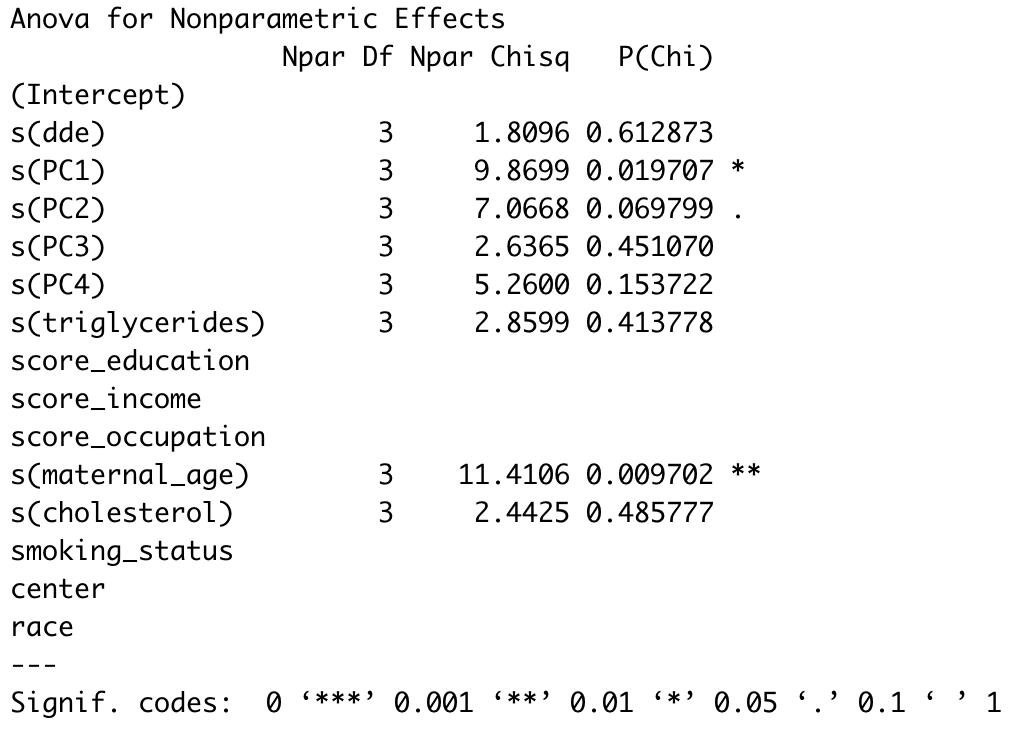
\includegraphics[width=10cm]{GAMOutputs2.png}
\end{frame}

\begin{frame}
\frametitle{GAM Outputs}
   \begin{minipage}{1\textwidth}
    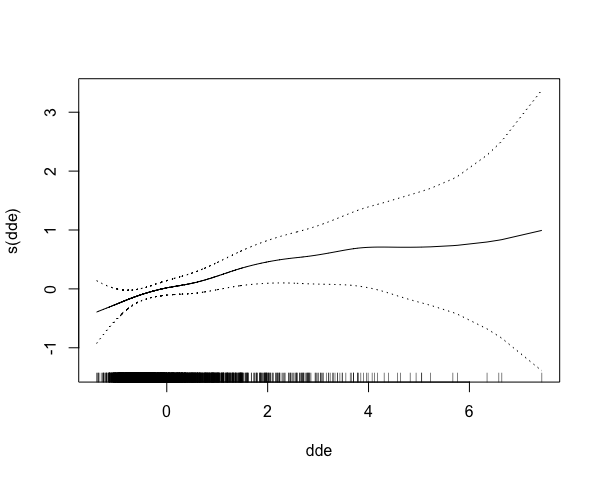
\includegraphics[width=55mm]{GAMPlotdde.png}
    \hfill
    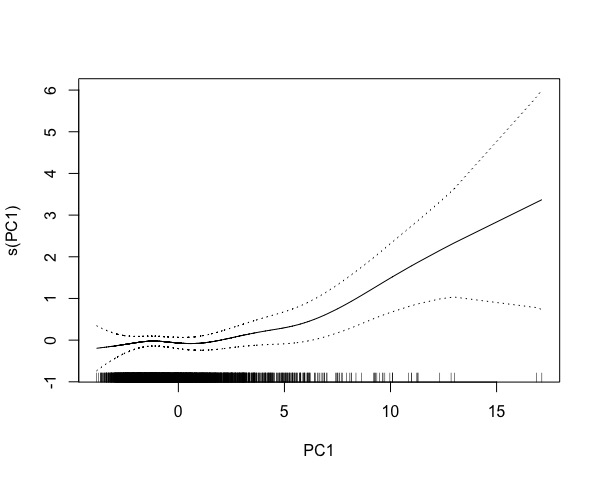
\includegraphics[width=55mm]{GAMPlotPC1.png}
    \vspace{0.5cm}
    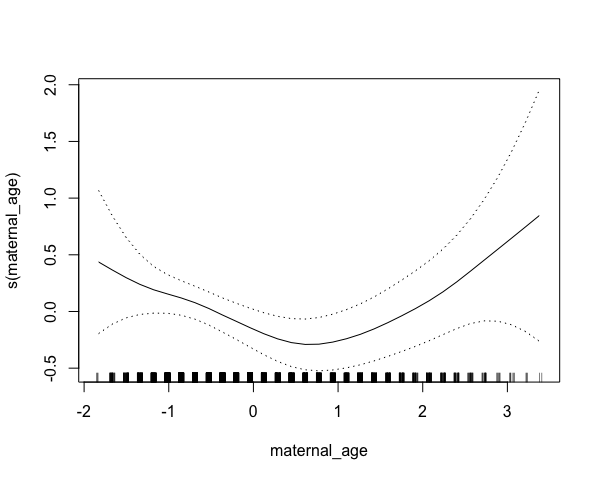
\includegraphics[width=55mm]{GAMPlotMaternalAge.png}
    \hfill
    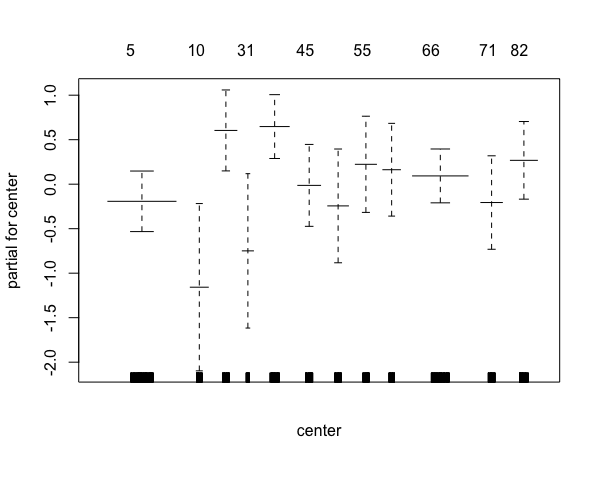
\includegraphics[width=55mm]{GAMPlotCenter.png}
  \end{minipage}
\end{frame}

\begin{frame}
\frametitle{Model}

\begin{itemize}

\item Frequentist approach may overestimate uncertainty.
\item Frequentist GAM may produce a non-significant p-value.
\pause
\item Bayesian Generalized Additive Model
$$g(Y_i) = \beta_0 + \sum_{j=1}^m f_j(x_{ij}) + \sum_{k=1}^l \beta_{k}z_{ik}$$

\item Adds priors on the common regression coefficients, priors on the standard deviations of the smooth terms.


\end{itemize}
\end{frame}

\begin{frame}
\frametitle{Model Results - align with frequentist model}
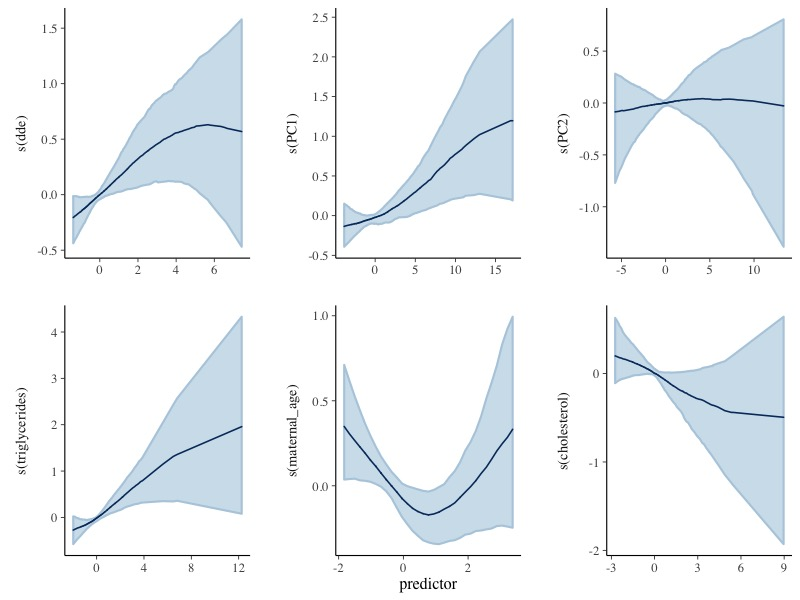
\includegraphics[width = 10cm]{BGAM.jpeg}
\end{frame}



\begin{frame}
\frametitle{Model Check}
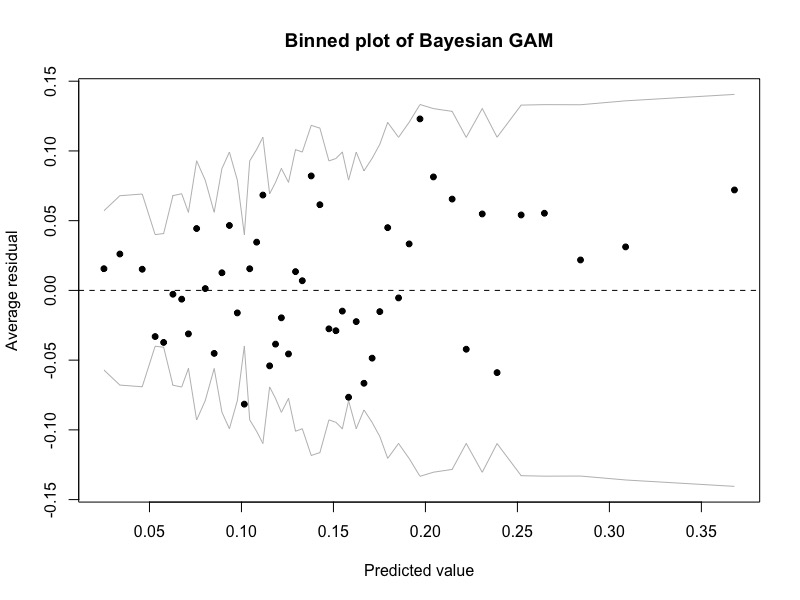
\includegraphics[width = 10cm]{BGAM2.jpeg}

\end{frame}














\begin{frame}
\frametitle{Discussion}



\begin{itemize}

\item Deal with different centers
\pause
\item Approach 1: Bayesian Hierarchical Model
\item Approach 2: Mixed Effect / Random Effect Model
\pause
\item Generalized Additive Mixed Model (GAMM)
\item Bayesian GAMM 


\end{itemize}
\end{frame}


\begin{frame}
\frametitle{Discussion}

\begin{itemize}

\item Specialized prior may give narrower credible intervals.
\pause
\item Including Interactions: Bayesian Factor Analysis (Ferrari, F. and Dunson, D.B. 2019)
\pause
\item Model with variable selection (e.g. LASSO, GAM + penalty)


\end{itemize}
\end{frame}









\end{document}
